\documentclass[11pt, twocolumn]{article}
\usepackage[left=1in, right=1in, top=1in, bottom=1in, includefoot]{geometry}		% Set margins to 1 inch.
\usepackage[utf8]{inputenc}

% Reduce the vertical space above the title.
\usepackage{titling}
\setlength{\droptitle}{-8ex}

\usepackage{amsmath}				% For \text{}

\usepackage{amsthm}				% For proof environment
\newtheorem{lemma}{Lemma}
\newtheorem{theorem}{Theorem}

\usepackage{amsfonts}				% For \mathbb{}

\usepackage{graphicx}
\usepackage[labelformat=simple]{subcaption}             % For the subfigure environment
\usepackage{floatrow}

\usepackage{nccmath}				% For fleqn environment

\usepackage{color}

\usepackage{bm}					% For \bm{}
\usepackage{physics}				% For \norm{}

\usepackage{enumerate}				% For customizing the numbering in the enumerate environment
%\usepackage{fitch}					% For Fitch-style proofs

\usepackage{tabularx}				% For making tables fit within page width
\usepackage{titlesec}				% For making the text of a section start on the same line as the section's title
\usepackage{url}					% For \url{}
\usepackage{hyperref}				% For breaking URLs
%\def\UrlBreaks{\do\/\do-}				% For breaking URLs at '/' and '-'
\usepackage{cleveref}				% When using hyperref, cleverref must be loaded after hyperref has been loaded.
\usepackage[T1]{fontenc}				% For fixing underscores in \url{}

% https://tex.stackexchange.com/questions/51682/is-it-possible-to-pagebreak-aligned-equations
\usepackage{IEEEtrantools}
\allowdisplaybreaks					% For allowing page breaks in aligned equations

\renewcommand\thesubfigure{(\alph{subfigure})}		% For adding parentheses around subfigure references (Figure 2(a) instead of Figure 2a)

\newcommand{\colvect}[2]{
	\ensuremath{\big[\begin{smallmatrix}#1\\#2\end{smallmatrix}\big]}
}

\newcommand{\longtabletext}[1]{
	\parbox[c]{\hsize}{\vspace*{1mm} #1 \vspace*{1mm}}
}

% The \vspace command inside the \title command is used to reduce
% the space between the title and the author lines.
\title{Explaining Predictions of Deep Neural Networks \\ on the Yelp Dataset}
\author{
	Caleb Kaiji Lu \\
	{\tt caleb.lu@sv.cmu.edu}
	\and
	Selva Samuel \\
	{\tt ssamuel@andrew.cmu.edu}
}
\date{}

%\hypersetup{draft}
\begin{document}

\maketitle

\section{Introduction}

In recent years, deep neural networks have been proposed to improve the effectiveness of neural networks in various machine learning tasks such as image classification, natural language processing, speech recognition, etc. However, the models learned by deep learning systems tend to be very complex and are not easily understandable by humans. This can be problematic when deep neural networks are used to make decisions that have a societal impact such as hiring, credit decisions, prison sentencing, etc. In such applications, it is necessary to check that the decision was made in a fair manner. For example, if an algorithm decides that a job offer should not be made then this decision should have been based on the basis of the candidate's lack of required skill and not on the basis of their gender or ethnicity.

The goal of our project is to generate explanations for predictions made by a deep neural network.

\section{Problem Statement}

In this project, we generate explanations for predictions made by a deep neural network that has been trained on the Yelp dataset \cite{Yelp2017}. We generate explanations for two prediction tasks: 1) Sentiment analysis, and 2) Gender prediction.

\subsection{Sentiment Analysis}

Yelp reviews are utilized by users to make decisions about which service provider (restaurants, doctors, etc.) to use for their needs. In making these decisions, users need to understand what aspects of the service provided is reflected in a reviewer's overall rating. For example, if a user is interested in a restaurant which has low ratings, they might need to understand if the low rating is because of bad food or some other aspect (such as ambience, etc.) which they do not care about. So, it is essential to enumerate the factors that contributed to a given reviewer's rating.

\subsection{Gender Prediction}

Recent advances in natural language processing have enabled the prediction of an author's gender from the text they have written by automatic analysis of linguistic characteristics of the text. We investigate the accuracy of deep neural networks in predicting the gender of a user based on the reviews that they have written. Again, it is important to understand which factors of the review text contribute towards making an accurate prediction. This would provide an understanding of what needs to be done to change the review text suitably in case a user wants to provide an anonymous review.


\section{Related Work}

A recurrent neural network (RNN) is a neural network which allows cyclical connections. Thus, recurrent connections allow a `memory' of previous inputs to persist in the network's internal state, which can then be used to influence the network output. Many varieties of RNNs have been proposed in the literature, such as Elman networks \cite{Elman1990}, Jordan networks \cite{Jordan1990}, time delay neural networks \cite{Lang1990}, etc.

In standard RNN architectures, the influence of a given input on the network output either decays or blows up exponentially as it cycles around the network's recurrent connections. This shortcoming is referred to as the \textit{vanishing gradient problem} \cite{Bengio1994}. The most effective solution so far to the vanishing gradient problem is the Long Short Term Memory (LSTM) architecture \cite{Hochreiter1997}.

Convolutional neural networks (CNNs) were developed to improve the effectiveness of pattern detection tasks in computer vision. They were inspired by the concept of receptive field \cite{Fukushima1988} in biological vision. The biological function can be approximated in computers using the convolution operation \cite{Marr1980}. A set of convolutional filters can be combined to form a \textit{convolutional layer} of a neural network.

In recent years, RNNs and CNNs have been used to perform a variety of natural language processing tasks. For example, in sentiment analysis tasks, most state-of-the-art methods \cite{Tang2015} use a combination of convolutional and recurrent neural networks. Convolutional neural networks, despite their use mainly in image-based applications, are also used in text-based applications which involve summarization of text since convolution can learn a holistic representation of a group of words instead of just individual words. Similar architectures of neural network models have been used in gender classification tasks as well \cite{Burger2011, Mukherjee2010}. However, none of these works generate explanations about why the model works well, or what kind of information is learnt by the system.


\section{Approach}

\subsection{Sentiment Analysis}

We trained a recurrent neural network on the Yelp review dataset to predict the ratings given by the users. We trained a binary classifier to categorize the reviews as positive or negative. If a review has a rating less than three stars, then we treat it as positive. Otherwise, we treat it as negative.

\subsubsection{Network Architecture}

The architecture of the deep neural network that we used is shown in figure \ref{fig:dnn-arch}. It consists of the following layers:
\\ \\
\textbf{(a) Embedding Layer.} We used an embedding layer whose input dimension was 20,000 and output dimension was 128. These values of the input and output dimensions are commonly used for embedding layers (see, for example, \cite{Lu2017}). We used the dropout technique \cite{ZarembaSV2014} to randomly zero 20\% of signals in the embedding layer.
\\ \\
\textbf{(b) Convolutional Layer.} We used a 1-dimensional convolutional layer with 64 filters. We used a 1-dimensional convolution window of length 5 and a stride of 1. We used the Rectified Linear Unit (ReLU) activation function for the convolutional layer.
\\ \\
\textbf{(c) Max Pooling Layer.} We used a max pooling layer with a pool size of 4 and a stride of 1.
\\ \\
\textbf{(d) LSTM Layer.} We used a long short-term memory (LSTM) layer with 128 units. We used the dropout technique \cite{ZarembaSV2014} to randomly zero 20\% of the rows in the weight matrices in the LSTM layer.
\\ \\
\textbf{(e) Sigmoid Activation Layer.} We used an activation layer that applies the sigmoid function to the outputs of the LSTM layer.
\\ \\
\textbf{(f) Loss Function.} We used the binary cross entropy loss function to generate prediction scores. In the sentiment analysis task, if the prediction score is less than 0.5, then the review text is classified as being negative. Otherwise, the review text is considered to be positive.

\subsubsection{Input Encoding}

The reviews are encoded as a sequence of word indices based on the overall frequency in the dataset. We set the maximum sequence sequence length to 300 among the top 20,000 most common words. Longer sequences were truncated while shorter ones were zero-padded.

\begin{figure*}[t]
	\includegraphics[width=\textwidth]{figure1}
	\caption{Architecture of deep neural network used for prediction tasks in the Yelp dataset}
	\label{fig:dnn-arch}
\end{figure*}

\subsection{Gender Prediction}
\label{subsection:gp}

We trained another recurrent neural network on the Yelp review dataset to predict the gender of the authors of the reviews and generated explanations for the predictions made by the network. For gender prediction, we used the same network architecture and input encoding as that for sentiment analysis. For the loss function, we deem the prediction to be female if the score is larger than 0.5, and male otherwise. 

\subsubsection{Ground Truth}

The Yelp dataset includes only the first names of the users who have written reviews and does not include their gender. So, we used the gender guesser tool \cite{GenderGuesser2017} to determine the gender of the review authors from their first names. When a first name is given as input to the gender guesser tool, the result is one of \texttt{male}, \texttt{female}, \texttt{mostly\char`_male}, \texttt{mostly\char`_female}, \texttt{andy} (the probability of being male is the same as the probability of being female) or \texttt{unknown} (the name was not found in the database used by the tool). We used only the reviews written by users for whom the gender guesser tool returned \texttt{male} or \texttt{female} (i.e., the tool was 100\% certain about the gender returned) for training our neural network.

\subsubsection{Single Reviews}

We trained two networks for gender prediction. In the first network, we used individual reviews for training our network.

\subsubsection{Combined Reviews}

Since single reviews are not very long, we also combined together all the reviews of a specific user in the dataset and used the combined reviews to train our network.

\subsection{Explanation Generation}

We used two methods to explain the predictions from our trained neural network - integrated gradients and masking. We explain both of these approaches in the following subsections.

\subsubsection{Integrated Gradients}

In order to generate explanations using integrated gradients, we adapted the method introduced by Sundararajan et al. \cite{Sundararajan2017}. In neural networks, gradients (of the output with respect to the input) can be used to explain the behavior of prediction tasks. However, gradients suffer from the weakness that if the prediction function flattens at the input, then the gradient would become zero. This causes a failure to highlight input features that are relevant to producing the observed output (see \cite{ShrikumarGK17} for details). Integrated gradients overcome this limitation of the gradient-based approach and provide a better way for generating explanations.

Suppose that $F: \mathbb{R}^n \to [0, 1]$ is a function that represents a deep neural network. Let $x \in \mathbb{R}^n$ be the input at hand and let $x' \in \mathbb{R}^n$ be the baseline input. For image networks, the baseline could be the black image, while for text models it could be the zero embedding vector. Then, the integrated gradient along the $i^{th}$ dimension for an input $x$ and baseline $x'$ can be calculated by using the following formula:
\begin{IEEEeqnarray*}{l}
    \mathsf{IntegratedGrads}_i(x) ::= \\
    \qquad (x_i - x_i') \times \int_0^1 \frac{\partial F(x' + \alpha \times (x - x'))}{\partial x_i} d\alpha
\end{IEEEeqnarray*}

Here, $\frac{\partial F(x)}{\partial x_i}$ is the gradient of $F(x)$ along the $i^{th}$ dimension. Thus, to compute integrated gradients, we consider the straightline path (in $\mathbb{R}^n$) from the baseline $x'$ to the input $x$, and compute the gradients at all points along the path. Integrated gradients are obtained by cumulating these gradients. In other words, integrated gradients are the path integral of the gradients along the straightline path from the baseline $x'$ to the input $x$.

As demonstrated in \cite{Sundararajan2017}, the integrated gradient metric performs well on a variety of classification tasks for images as well as text input.

\subsubsection{1-gram Masking}

The second method that we used to generate explanations of predictions made by our trained neural network is 1-gram masking. In natural language processing, an n-gram refers to a contiguous sequence of n words in a piece of text. So, 1-gram is just a single word. In 1-gram masking, the importance of a word in making a correct prediction is determined by the magnitude of the change in the prediction score when all occurrences of the word are removed from the text. The larger the change in the prediction score, the greater is its influence on making the correct prediction.


\section{Results}

We used the Keras\footnote{\url{https://keras.io}} deep learning framework for implementing our neural networks. Keras is a high-level deep learning framework. It can use Theano\footnote{\url{http://deeplearning.net/software/theano/}} or TensorFlow\footnote{\url{https://www.tensorflow.org}} as its backend. We ran Keras on top of TensorFlow.

We used a server with a 64-bit Intel Xeon processor and 128GB RAM for training our networks. The training process took about 20 minutes for the sentiment analysis task and 60 minutes for the gender prediction task.

\subsection{Sentiment Analysis}

We trained our network for sentiment analysis with 200,000 reviews. We kept the labels balanced in our training set so that the number of reviews with positive ratings was the same as the number of reviews with negative ratings.

\subsubsection{Prediction Accuracy}

For our implementation, although our end goal was not to train a classifier that beat the best method for this dataset, we still wanted our model be as close to the best method as possible. The best accuracy so far for sentiment analysis on this data set has been 96\% \cite{Tang2015}. We were able to train a model whose validation accuracy is 93\%.

\subsubsection{Explanations Generated}

We generated explanations for the predictions made by our network for sentiment analysis using integrated gradients and 1-gram masking. Figure \ref{fig:sa:int-grad} shows examples of explanations generated by using integrated gradients. In particular, figure \ref{fig:sa:int-grad:pos} shows the explanations generated for a positive review and figure \ref{fig:sa:int-grad:neg} shows the explanations generated for a negative review. In figure \ref{fig:sa:int-grad:pos}, the words ``the'' and ``is'' have been assigned relatively lower weights while the words ``food'' and ``amazing'', which are words more central to the positive sentiment of this sentence, have been assigned higher weights. Similarly in figure \ref{fig:sa:int-grad:neg}, words such as ``really'', ``hate'' and ``tastes'' have been assigned higher weights than the other words because they 
have a higher influence in causing this review to be negative.

Figure \ref{fig:sa:mask} shows examples of explanations generated by using 1-gram masking. More specifically, figure \ref{fig:sa:mask:neg} shows the explanations generated for a negative review and figure \ref{fig:sa:mask:pos} shows the explanations generated for a positive review. The red horizontal line in these figures shows the prediction score for the complete review text without any of the words being masked. As words in the review text are masked, the prediction score changes. The prediction score obtained by masking a particular word is shown by the bar corresponding to that word. Words which cause a higher change in the prediction score are more central to determining the sentiment associated with the review text. Thus, the word ``disappointing'' has a higher relevance for explaining the negative sentiment in figure \ref{fig:sa:mask:neg}. Similarly, in figure \ref{fig:sa:mask:pos}, the word ``great'' (whose masking causes the greatest drop in the prediction score) is the most relevant for explaining the positive sentiment in the review. 

\begin{figure*}[t]
	\centering
	\begin{subfigure}{0.45\textwidth}
		\centering
		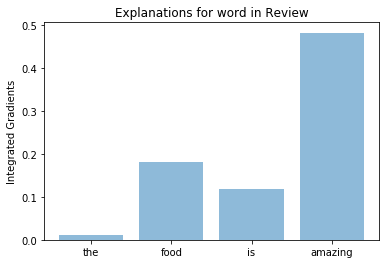
\includegraphics[width=\linewidth]{figure2}
		\caption{Positive review}
		\label{fig:sa:int-grad:pos}
	\end{subfigure} % There should be no newlines here.
	\begin{subfigure}{0.45\textwidth}
		\centering
		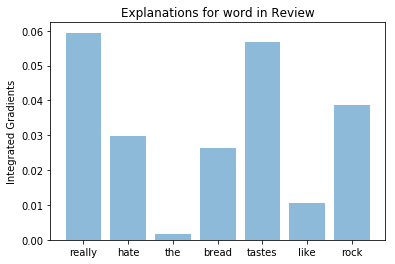
\includegraphics[width=\linewidth]{figure3}
		\caption{Negative review}
		\label{fig:sa:int-grad:neg}
	\end{subfigure}
	\caption{Explanations generated for sentiment analysis by using integrated gradients}
	\label{fig:sa:int-grad}
\end{figure*}

\begin{figure*}[t]
	\centering
	\begin{subfigure}{0.45\textwidth}
		\centering
		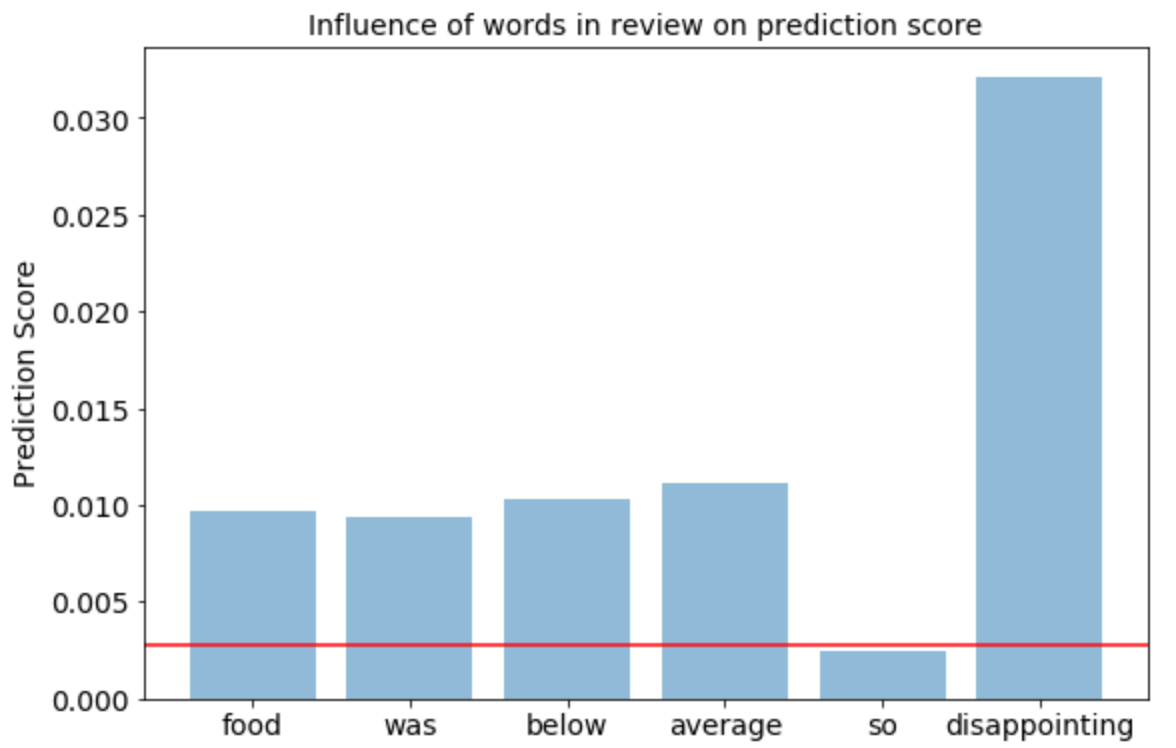
\includegraphics[width=\linewidth]{figure5}
		\caption{Negative review}
		\label{fig:sa:mask:neg}
	\end{subfigure} % There should be no newlines here.
	\begin{subfigure}{0.45\textwidth}
		\centering
		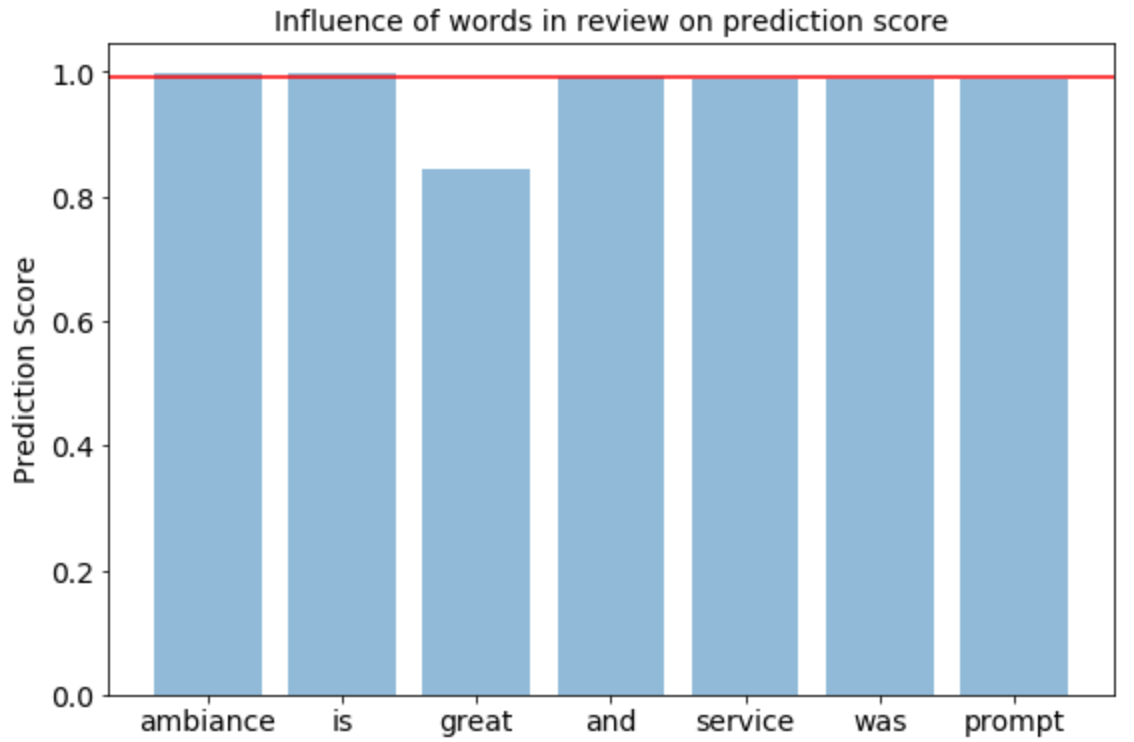
\includegraphics[width=\linewidth]{figure4}
		\caption{Positive review}
		\label{fig:sa:mask:pos}
	\end{subfigure}
	\caption{Explanations generated for sentiment analysis by using 1-gram masking}
	\label{fig:sa:mask}
\end{figure*}

\subsection{Gender Prediction}

 As mentioned in section \ref{subsection:gp}, we trained two networks for gender prediction - one with individual reviews and the other with reviews of particular users combined together. We used 500,000 reviews for training the network for gender prediction using single reviews. We trained the network for gender prediction on combined reviews using 50,000 instances. In both cases, we kept the labels in our training set balanced. In other words, the number of instances corresponding to male reviewers was the same as the number of instances corresponding to female reviewers.

\subsubsection{Prediction Accuracy}

We achieved a classification accuracy of 69.5\% for single reviews, and 84.5\% for combine reviews. This is comparable to the accuracy of state-of-the-art neural networks that have been used to predict the gender of authors of blog posts and tweets \cite{Burger2011, Mukherjee2010}.

\subsubsection{Explanations Generated}

As in sentiment analysis, we used integrated gradients and 1-gram masking to generate explanations for the gender prediction task as well. Figure \ref{fig:gp:int-grad} shows examples of explanations generated by using integrated gradients. The integrated gradients with respect to each word in a review text written by a female reviewer is shown in figure \ref{fig:gp:int-grad:female}. The word ``nail'' is the most prominent word in this review. Similarly, figure \ref{fig:gp:int-grad:male} shows the integrated gradients with respect to each word in a review given by a male reviewer. The word ``wife'' is the most influential for explaining the prediction for this review.

Figure \ref{fig:gp:mask} shows examples of explanations generated by using 1-gram masking. In particular, figure \ref{fig:gp:mask:female} shows the changes in the prediction score caused by masking each word in a review given by a female reviewer. In this case, the prediction of the original review text is greater than 0.5 (shown by the horizontal red line). The masking of the word ``nails'' causes the largest drop in the prediction score. So, it is the most influential word that causes this review to be classified as written by a female person. Similarly, figure \ref{fig:gp:mask:male} shows the changes in the prediction score brought about by the masking of each word in a review written by a male reviewer. The prediction score of the original review text, in this case, is less than 0.5. The largest increase in the prediction score is caused by the masking of the word ``girlfriend''. Therefore, it is the most influential word in determining the gender of the writer of this review.

It is interesting to note that in all of the above examples, the neural network used semantic content of the review (e.g. women visit nail salons, men have wives or girlfriends, etc.) to determine if a reviewer was male or female.

\begin{figure*}[t]
	\centering
	\begin{subfigure}{0.45\textwidth}
		\centering
		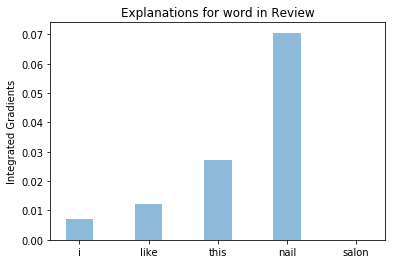
\includegraphics[width=\linewidth]{figure9}
		\caption{Female reviewer}
		\label{fig:gp:int-grad:female}
	\end{subfigure} % There should be no newlines here.
	\begin{subfigure}{0.45\textwidth}
		\centering
		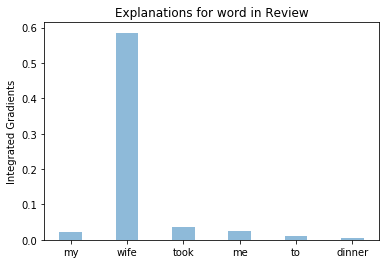
\includegraphics[width=\linewidth]{figure8}
		\caption{Male reviewer}
		\label{fig:gp:int-grad:male}
	\end{subfigure}
	\caption{Explanations generated for gender prediction by using 1-gram masking}
	\label{fig:gp:int-grad}
\end{figure*}

\begin{figure*}[t]
	\centering
	\begin{subfigure}{0.45\textwidth}
		\centering
		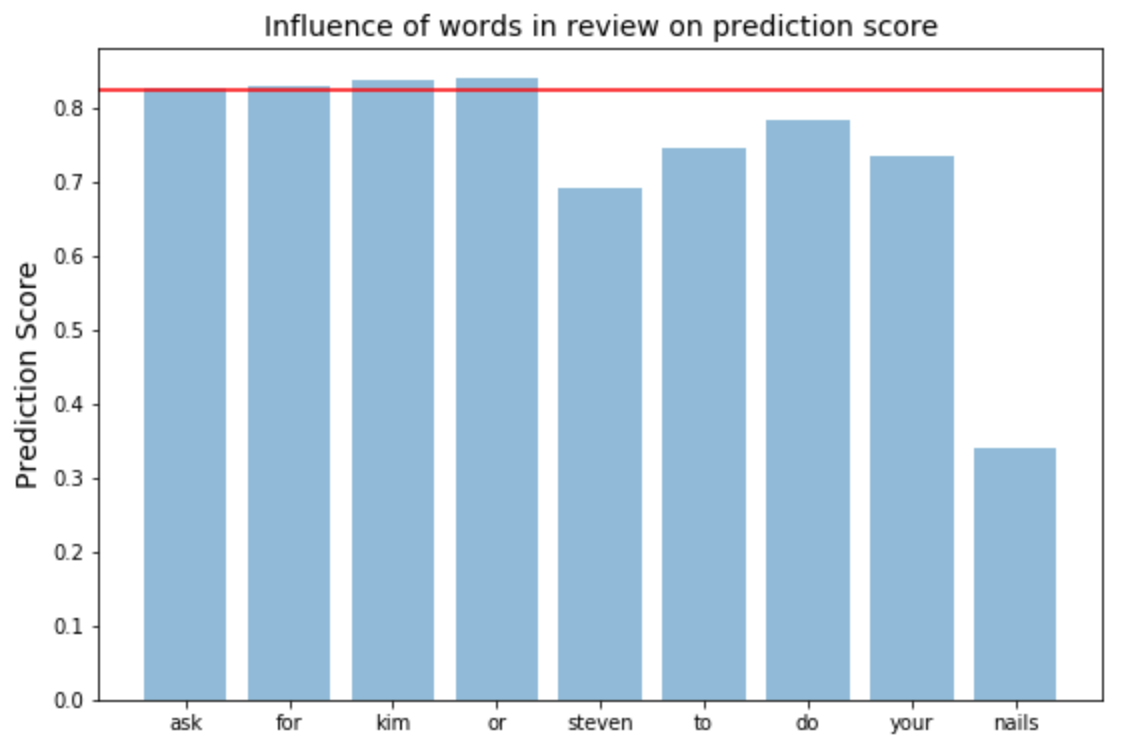
\includegraphics[width=\linewidth]{figure7}
		\caption{Female reviewer}
		\label{fig:gp:mask:female}
	\end{subfigure} % There should be no newlines here.
	\begin{subfigure}{0.45\textwidth}
		\centering
		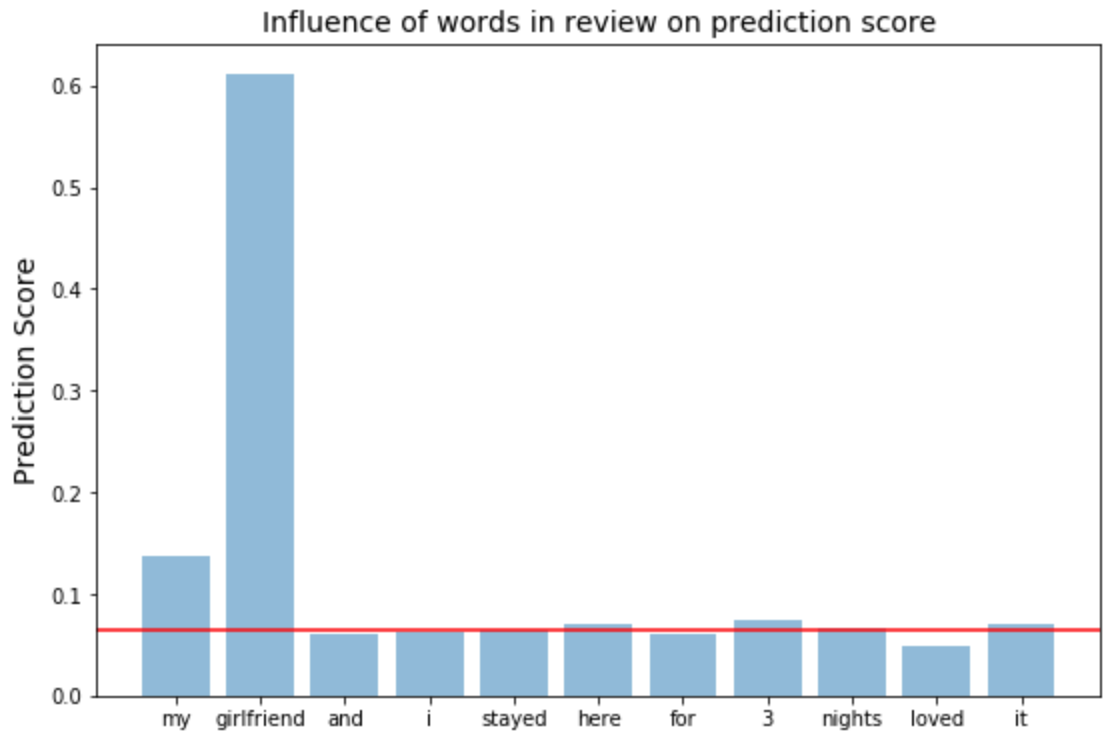
\includegraphics[width=\linewidth]{figure6}
		\caption{Male reviewer}
		\label{fig:gp:mask:male}
	\end{subfigure}
	\caption{Explanations generated for gender prediction by using 1-gram masking}
	\label{fig:gp:mask}
\end{figure*}

\subsubsection{Gender Bias}

We also tested the networks that we trained for gender prediction to see if they could detect stylistic differences between reviews from men and those written by women. We found some interesting examples of stylistic differences in the Yelp dataset. Table \ref{table:bias} shows an example in which the model exhibits gender bias by assigning higher probabilities to sentences with phrases like ``oh my god'' or ``sooooo'' causing the review to be classified as written by a female reviewer. The biases are likely learned by the system from similar instances in the training data that are written by female reviewers.

In figure \ref{fig:bias}, using the integrated gradients method, we can see that the word ``soooo'' is the most influential word in causing the sentence to be classified as written by a female person. This indicates that the model we have trained exhibits gender bias.

\begin{table*}
    \centering
    \begin{tabular}{|l|l|}
    \hline
    Review Text & Prediction Score  \\
    \hline
    'the food is good' & 0.49949434 (Male)  \\
    \hline
    'Oh my god the food is good' & 0.56273288 (Female)    \\
    \hline
    'Oh my god the food is sooooo good' & 0.75836354 (Female) \\
    \hline
    'Oh my god the food is sooooo good! I love this place!!' & 0.84929174 (Female)   \\
    \hline
    \end{tabular}
    \caption{Gender bias exhibited by the system}
    \label{table:bias}
\end{table*}

\begin{figure}
	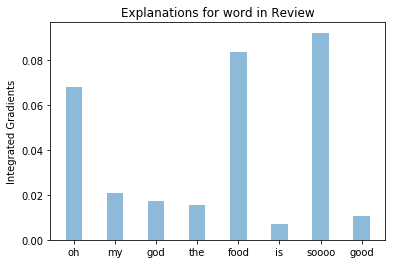
\includegraphics[width=\textwidth]{figure10}
	\caption{Explanation of Gender Bias}
	\label{fig:bias}
\end{figure}

\subsection{Effectiveness of Explanation Methods}

Despite the above results, the explanation models that we have used, namely integrated gradients and 1-gram masking, did not work well for all sentence instances that we tested. For example, integrated gradients does not work well when the review text is longer than a few words. The reason for this is that the points along the path from a baseline embedding vector to the actual embedding vector of a word are not in the distribution of an embedding at all. This is because all word embedding vectors are normalized to be on the radius-1 ball in the embedding space. So, if we normalize the points on the path, we essentially get the same vector; if we don't normalize it, we get vectors that are not in the distribution at all. As a result, integrated gradients used in an RNN language model may not perform as well as it does in image-related tasks.

The performance of 1-gram masking also varies greatly with the sentence or task. Often, there is a collection of words such that masking individual words does not change the prediction score much but masking them all introduces a significant change in the prediction score. Moreover, the order of words in a review text is also important. In addition, removing a word will necessarily break the distribution faithfulness since the sentence will likely become ungrammatical. Because of these reasons, simply removing a word will not necessarily create a good counter-factual for the sentence with regard to that word. 1-gram masking worked well in our examples because a single word had a large influence in making a prediction and masking it caused a drastic change in the prediction score. In gender prediction, for example, words such as ``husband'', ``wife'' and ``nails'' are semantically influential words in determining the reviewer's gender and exert a large influence on the prediction score. These words are stronger hints than stylistic word choices, thus accumulating most of the influence, thereby causing the explanation models to work really well.

In addition to integrated gradients and 1-gram masking, we also explored the use of \textit{Quantitative Input Analysis (QII)} \cite{Datta2017} for explaining machine learning models. QII uses a similar causal intervention mechanism as integrated gradients. It randomly intervenes on a single input or on multiple inputs by sampling from their distribution. It then inspects the influence of each input by looking at the outputs in relation to the casual intervention. However, it is hard to obtain a distribution for a single word in a sentence context. If we define the distribution based on the distance from the embedding vector, words that are close together can have a huge difference in the influence on the prediction for a sentence. For example, in the sentence \textit{The food is tasty}, if we intervene on the word \textit{tasty}, we can get both \textit{nasty} and \textit{delicious}, which are both close to the word \textit{tasty} in the embedding space. But we can expect these two interventions to have totally different outcomes. Thus, it is difficult to generate counterfactuals for words in a sentence, as the distribution of words in the embedding space is not always the ideal distribution for a certain task.


\section{Conclusion}

In this project, we used deep neural networks to perform two classification tasks on the Yelp dataset: sentiment analysis and gender prediction. For these tasks, we achieved a prediction accuracy that is comparable to that of state-of-the-art machine learning models that have been used for these tasks. We tried to explain the models using some two functional methods, namely integrated gradients and 1-gram masking. We found that these methods are not robust enough to always generate good explanations. An important challenge in using these methods lies in generating good counterfactuals that can be used to causally intervene the model. In the gender prediction task, we also found that the model picked up gender bias towards female reviewers, which causes potential privacy concerns.


\section{Project URL}

The source code of our project is hosted on GitHub at \url{https://github.com/selvasamuel/18734-project}.

\section{Work Distribution}

Caleb: Background research, designing and training the models, integrated gradient implementation, writing reports and making slides
\\ \\
Selva: Background research, preprocessing the dataset, 1-gram masking implementation, writing reports and making slides


\nocite{Lu2017}
\nocite{Sundararajan2017}
\nocite{ZarembaSV2014}
\nocite{Burger2011}
\nocite{Datta2017}
\nocite{Mukherjee2010}
\nocite{Ribeiro2016}
\nocite{Tang2015}
\nocite{Yelp2017}

\bibliographystyle{abbrv}
\bibliography{references}

\end{document}
